\section{Introduction}%
\label{sec:introduction}

Robots increasingly populate dynamic environments. 
% Motivation
Imagine a robot
operating alongside customers in a supermarket. It is requested to perform different
tasks, such as cleaning the floor or picking a wide range of products.
These different manipulation tasks may vary in their dimension
and accuracy requirements, e.g. rotation around a suction gripper
does not need to be specified while two-finger grippers require full poses. Thus,
it is important for motion planning algorithms to support various goal definitions.
Further, the robot is operating alongside humans, it has to constantly react to
the changing environment and consequently update an initial plan.
As customers move fast, the adaptations must be
computed in real time.
% Problem
Therefore, motion planning is often divided into global motion
planning~\cite{Karaman2011} and local motion planning, which we will refer
to as motion generation in this paper. A global planner
generates a first feasible path that is used by a motion generator as global guidance.
This paper proposes a novel approach to motion generation, that deals
with a variety of different goal definitions. 

%1) intro optimization based
Motion generation is often solved by formulating an optimization problem 
over a time horizon. The popularity of this approach is partly thanks to
the guaranteed collision avoidance and thus safety~\cite{Hrovat2012,hewing2020learning}.
The optimization problem is then assembled from a scalar objective
function, encoding the motion planning problem (e.g., the desired final position, path
constraints, etc.), the transition function, defining the robot’s
dynamics, and several inequality constraints, integrating physical limits and
obstacle avoidance. 
%
\begin{figure}[h]
  \centering
  \begin{subfigure}{0.5\linewidth}
    \centering
    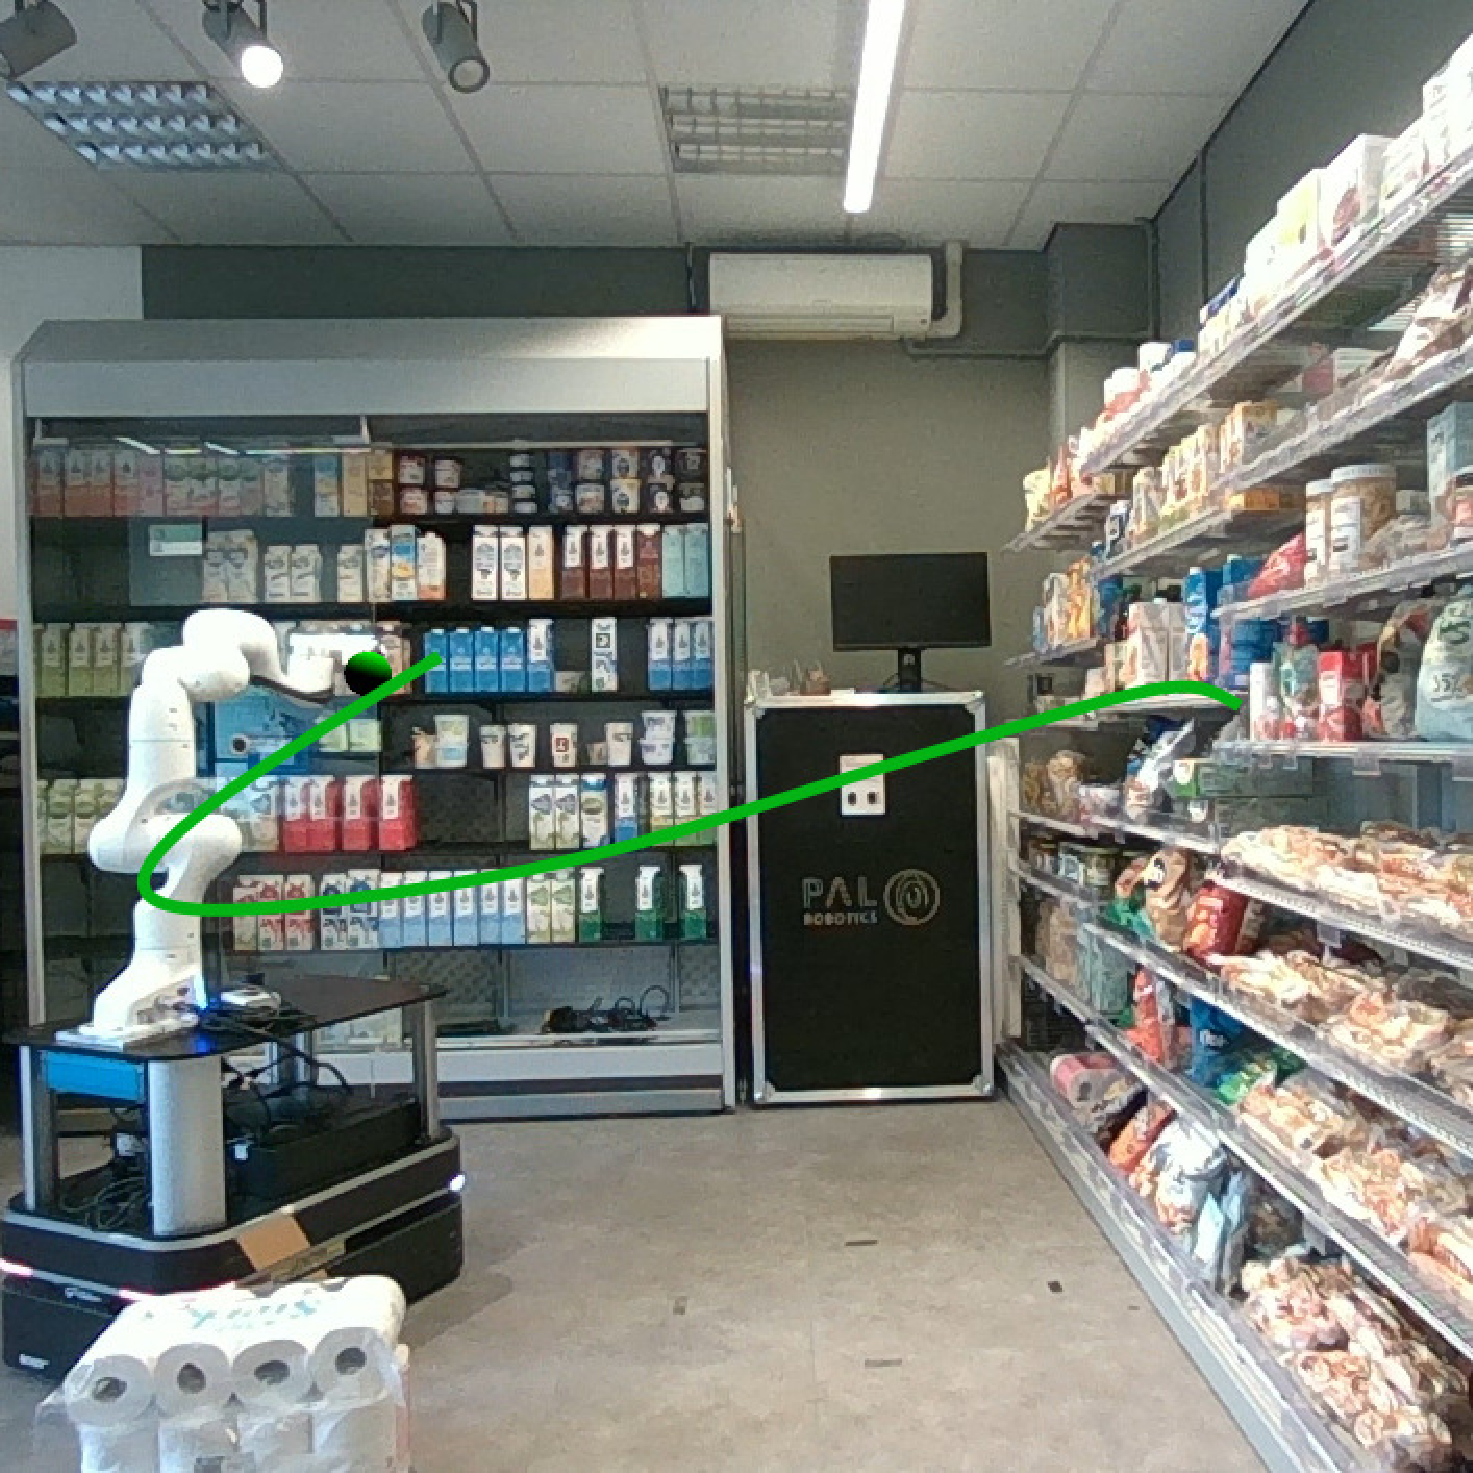
\includegraphics[width=0.9\textwidth]{4_non_holonomic/realAlbert/albert_spline_1}
    \caption{}
    \label{subfig:albert_spline_1}
  \end{subfigure}%
  \begin{subfigure}{0.5\linewidth}
    \centering
    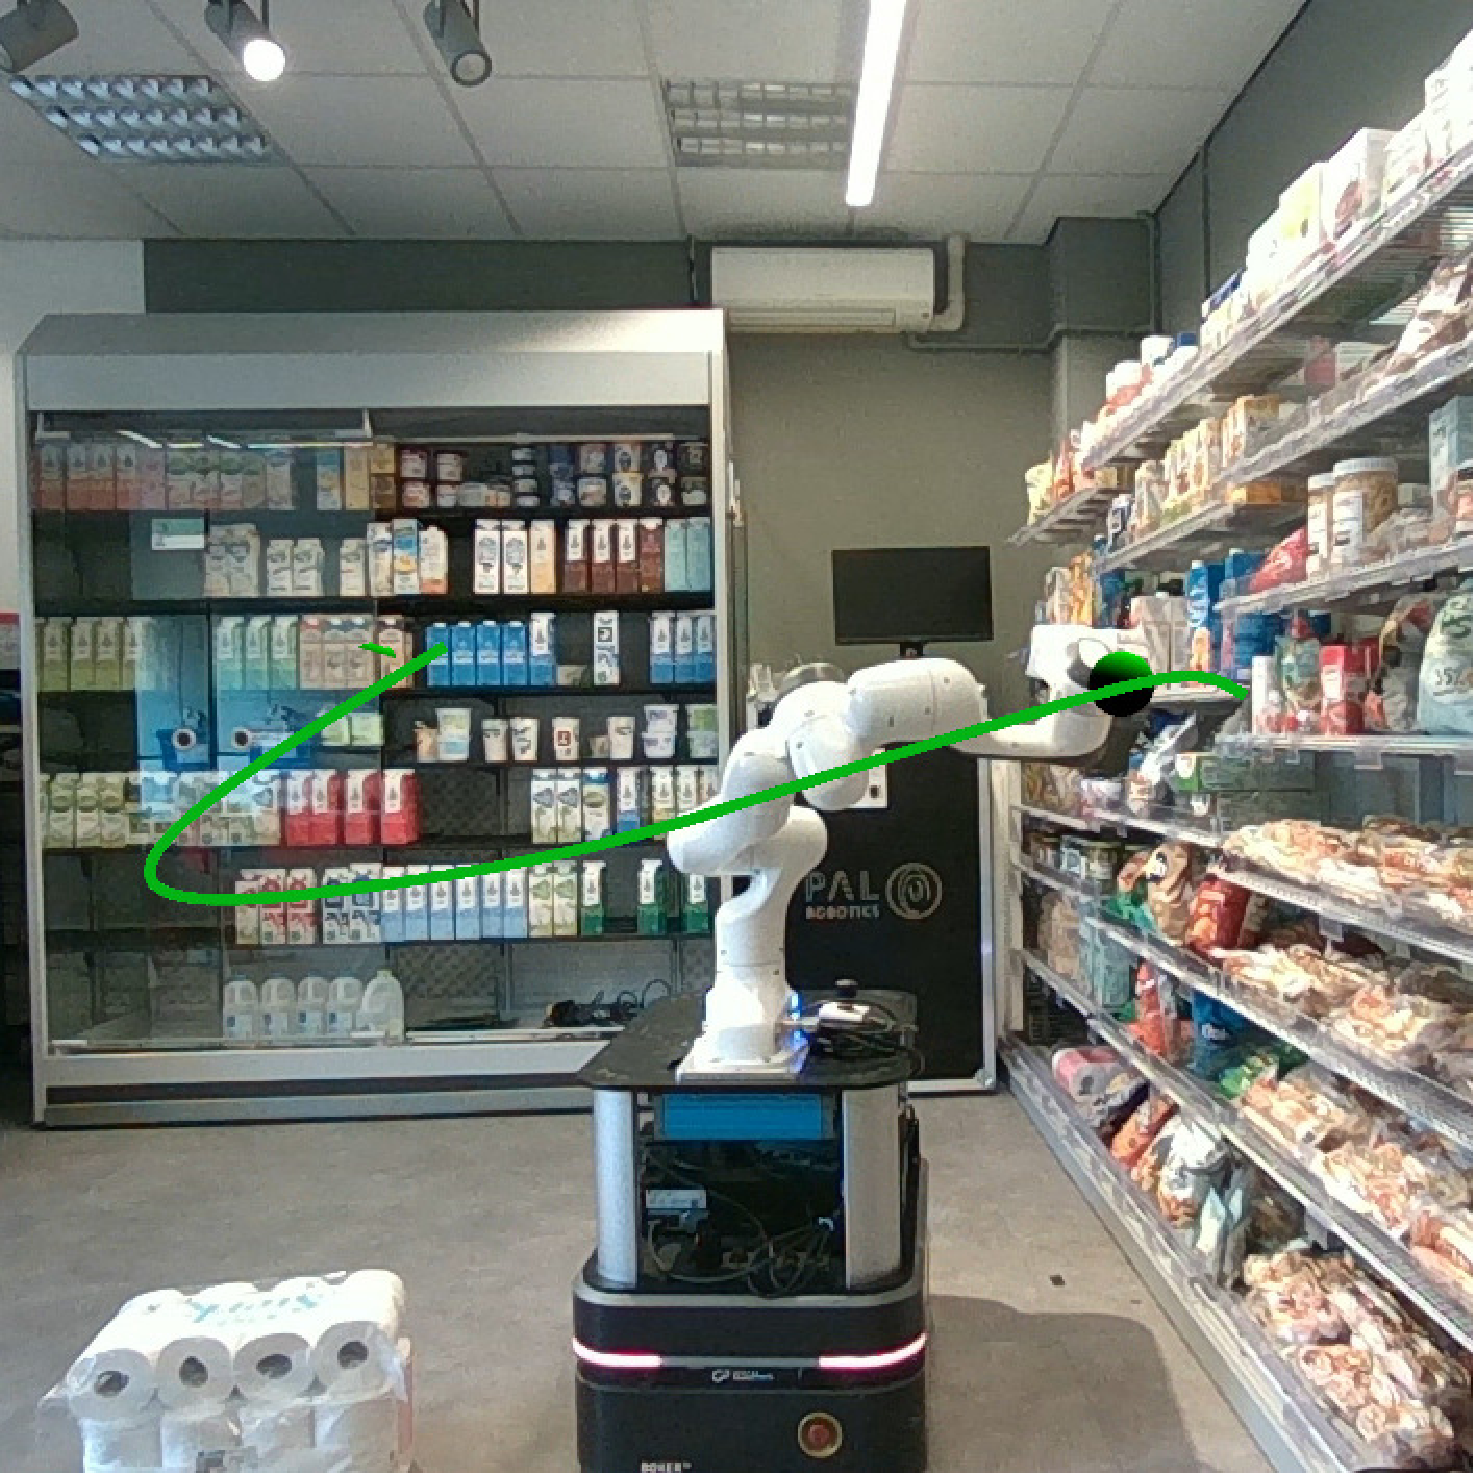
\includegraphics[width=0.9\textwidth]{4_non_holonomic/realAlbert/albert_spline_2}
    \caption{}
    \label{subfig:albert_spline_2}
  \end{subfigure}%
  \caption{
    Dynamic fabrics for path (green) following with a non-holonomic mobile
    manipulator. Dynamic fabrics control all actuators simultaneously to follow
    the end-effector path while keeping a given orientation and avoiding collision
    with the environment.
  }
  \label{fig:albert_spline_example}
\end{figure}
%
%2) drawbacks optimization based
Despite abundant applications of such optimization-based approaches
to mobile robots, the computational costs limit applicability when dealing with
high-dimensional configuration spaces~\cite{Bednarczyk2020,Richter2010}.
Data-driven approaches to speed up the optimization process usually come with
reduced generalization abilities, loss of formal
guarantees~\cite{hewing2020learning}
and require prior, often
costly, data acquisition. Moreover, due to the scalar objective function, the
user must carefully weigh up different parts of the objective function. As
a consequence, optimization-based approaches are challenging to tune and
inflexible to generic motion planning problems with variable goal
objectives~\cite{Xie2020,Edwards2021}. 

%3) intro fabrics
In the field of geometric control, namely Riemannian
motion policies (RMP) and optimization fabrics, all individual parts of the motion planning
problem are formulated as differential equations of second order.
Applying operations from differential geometry, the individual
components are combined in the configuration space to define the
resulting motion~\cite{Cheng2018,Ratliff2020}. This allows to iteratively
\textit{design} the motion of the robot while maintaining explainability over the resulting
motion~\cite{Cheng2018,Ratliff2020,Xie2020,Wyk2022}.

% Contribution statements
These works on optimization fabrics~\cite{Ratliff2020}, but also on
predecessors, such as RMP~\cite{Cheng2018} and RMP-Flow~\cite{Cheng2020},
have shown the power of designing reactive behavior as second-order
differential equations. However, integration of dynamic features, such as
moving obstacles and path following, have not been proposed
nor have the framework been applied to non-holonomic systems.
In this article, we exploit relative coordinate systems in the framework of
optimization fabrics by introducing the dynamic pullback operation (\cref{eq:dynamic_pull}).
This generalization 
can then integrate moving obstacles and path following.
We show that our generalization maintains
guaranteed convergence for path following tasks and improves collision
avoidance with moving obstacles.
Moreover, we propose a method
to incorporate non-holonomic constraints.
Lastly, we compare a trajectory optimization formulation, namely a model
predictive control formulation, with optimization fabrics to provide the reader
with a better understanding of key differences between the two approaches.
We analyze computational costs and the quality of resulting trajectories
for different robots.
%
Several simulated results and real-world experiments
show the practical implications of \ac{df}. The contributions of this paper can be
summarized as:

%Finally, we hypothesize
%that dynamic fabrics may lead to novel approaches to the global motion planning problem. 

\begin{enumerate}
  \item We enable the usage of optimization fabrics for dynamic scenarios.
    Specifically, we propose time parameterized differential maps using up-to
    second-order predictor models. As a consequence, this enables the
    integration of moving obstacles and path following tasks
    , see \cref{fig:reference_trajectory}.
  \item We extend the framework of optimization fabrics to non-holonomic robots.
  \item We present a quantitative comparison between model predictive control and
  optimization fabrics. The results reveal that fabrics are an order of magnitude faster,
  more reliable, and easier to tune for goal-reaching tasks with a robotic manipulator in
  static environments.
\end{enumerate}
All findings are supported by extensive experiments in both simulation and real-world
with a manipulator, a differential drive robot, and a mobile manipulator.
